%%%%%%%%%%%%%%%%%%%%%%%%%%%%%%%%%%%%%%%%%%%%%%%%%%%%%%%%%%%%%%%%%%%%%%%%%%%%%%%%%%%%%%%%%%%%%%%%%%%%%%
%
%   Filename    : chapter_6.tex 
%
%   Description : This file will contain 
%                 
%%%%%%%%%%%%%%%%%%%%%%%%%%%%%%%%%%%%%%%%%%%%%%%%%%%%%%%%%%%%%%%%%%%%%%%%%%%%%%%%%%%%%%%%%%%%%%%%%%%%%%

\chapter{Cycling Segment Dataset}

This chapter presents a comprehensive description of the dataset produced through the WeCyclePH platform. This dataset captures detailed, segment-level information on urban cycling experiences, derived from both user-generated and machine-generated data. By combining GPS traces, real-time annotations, and computer vision outputs, we construct a GeoJSON-based spatial dataset that supports diverse applications in mobility research, infrastructure evaluation, and participatory urbanism.

Rather than abstracting entire rides into coarse summaries, our approach decomposes rides into route segments based on directional continuity. Each segment becomes a standalone analytical unit represented as a \texttt{Feature} within a valid GeoJSON \texttt{FeatureCollection}, complete with geometry, spatiotemporal metrics, and annotation metadata. This allows stakeholders to conduct fine-grained spatial analysis while remaining grounded in real cyclist experiences.

\section{Dataset Overview}
The dataset is organized around the principle of route segmentation. Each ride is split into segments based on directional stability. A segment is a continuous path represented as a GeoJSON Feature with rich metadata about cyclist activity and experience. These segments are collected into a GeoJSON FeatureCollection.

Each segment Feature contains:
\begin{itemize}
\item \texttt{geometry}: a LineString defining the coordinates of the segment.
\item \texttt{properties}: metadata including distance, duration, average speed, elevation gain, and time range.
\item \texttt{annotation\_summary}: a normalized summary of annotation types encountered.
\item \texttt{annotations}: an optional list of full annotation objects, including sentiment, tags, media, and coordinates.
\end{itemize}

\section{Structure and Design Philosophy}

GeoJSON was selected as the primary format due to its wide support in geographic information systems (GIS), web-based mapping tools, and data science workflows. Each segment is encoded as a 	exttt{Feature}, and all segments are wrapped into a 	exttt{FeatureCollection}. Each feature has:

\begin{itemize}
    \item a \texttt{geometry} field of type \texttt{LineString}, representing the segment's path.
    \item a \texttt{properties} object containing metadata about the segment.
    \item an optional \texttt{annotations} array with detailed feedback or observations.
    \item a derived \texttt{annotation\_summary} summarizing types of annotations per segment.
\end{itemize}

Every feature is a composite unit that brings together objective measurements (distance, speed, elevation gain) and subjective inputs (annotations and sentiment), reflecting the dual nature of cyclist experience.


\section{Data Sources}

\subsection{GPS and Ride Metadata}
Each recorded ride consists of a sequence of timestamped GPS points, optionally including elevation. These are collected via the WeCyclePH mobile application. Each point has the following structure:
\begin{figure}[H]
\centering
\begin{lstlisting}[language=json, label={lst:feature_pointstructure}]
{
    "coordinate: {
        "latitude": number,
        "longitude": number
    },
    "timestamp": integer,     // milliseconds since epoch
    "elevation": number       // meters above sea level
}
\end{lstlisting}
\caption{Structure of recorded GPS points}
\label{fig:PointStructure_Feature}
\end{figure}
GPS points form the backbone of the dataset and are used to calculate distances, speeds, elevation gains, and route geometries.

\subsection{User Annotations}
Cyclists can annotate their rides with comments, experiences, and descriptive tags. Each annotation is linked to one or more GPS coordinates and may include media such as images or videos. An example structure:
\begin{figure}[H]
\centering
\begin{lstlisting}[language=json, label={lst:feature_annotation}]
{
    "id": string,
    "type": string,              // e.g., "obstruction", "comfort"
    "sentiment": string,         // free-form input
    "annotationLabel": string,   // predefined label
    "createdAt": string,         // ISO datetime
    "points": [
        {
            "coordinate": {"latitude": number, "longitude": number},
            "timestamp": integer
        },
        ...
    ],
    "mediaUri": string,          // optional URI to Cloud Storage
    "mediaType": string,         // e.g., "image", "video"
    "additionalTags": [string]
}
\end{lstlisting}
\caption{Data structure of a user annotation in WeCyclePH, showing fields for annotation type, sentiment, predefined label, geospatial coordinates with timestamps, optional media attachments, and additional tags.}
\label{fig:AnnotationStructure_Feature}
\end{figure}
Annotation labels are standardized for analysis. Valid predefined annotation labels include: \texttt{bike-lane, shared-road, no-bike-lane, barrier-bollard, obstruction, pothole, rough-surface, smooth-surface, steep-incline, steep-decline, rest-stop, construction, intersection, bike-shop, traffic-high, traffic-low, media-annotation}. These annotations are used both for qualitative insight and quantitative summary.

\section{Segment Feature Format}
Each recorded ride in the WeCyclePH dataset is subdivided into multiple segments, each represented as a GeoJSON Feature. This segmentation enables fine-grained analysis of route conditions and cyclist experiences along different portions of the ride. The use of GeoJSON was chosen for its compatibility with mapping platforms and geospatial analysis tools such as Mapbox, Leaflet, and GIS libraries. Each segment encodes spatial geometry, temporal boundaries, computed metrics, and annotation information.

\subsection{Feature Format}
Figure~\ref{fig:Feature_Format} presents the canonical structure of a segment feature in GeoJSON format. Each feature contains a \texttt{LineString} geometry representing the route segment and a \texttt{properties} object that stores metadata.
\begin{figure}[H]
\centering
\begin{lstlisting}[language=json, label={lst:feature_format}]
{
    "type": "Feature",
    "geometry": {
        "type": "LineString",
        "coordinates": [[lng, lat], ...]
    },
    "properties": {
        "ride_id": string,
        "start_time": integer,
        "end_time": integer,
        "distance": number,
        "duration": number,
        "elevation_gain": number,
        "average_speed": number,
        "annotation_summary": {
            [annotation_label]: number
        },
        "annotations": [ ... ]
    }
}
\end{lstlisting}
\caption{GeoJSON feature format for a ride segment in WeCyclePH, containing a LineString geometry for the route and metadata properties such as ride details, performance metrics, and associated annotations.}
\label{fig:Feature_Format}
\end{figure}

\subsection{Feature Examples}

\paragraph{Feature Without Annotations.} Not all route segments carry explicit user annotations. Nevertheless, such segments are valuable for capturing continuous ride metrics such as speed, elevation, and route geometry. Figure~\ref{fig:SampleFeature_NoAnnotation} shows an example of a minimal segment feature without any annotations. It includes geometry and performance metrics, which remain useful for understanding baseline cycling conditions or empty stretches of the route.
\begin{figure}[H]
\centering
\begin{lstlisting}[language=json, label={lst:feature_none}]
{
  "type": "Feature",
  "geometry": {
    "type": "LineString",
    "coordinates": [
      [121.0503095, 13.7654465],
      [121.0503301, 13.7654397]
    ]
  },
  "properties": {
    "ride_id": "1djehOENxM2m4dACbmjy",
    "start_time": 1752572589205,
    "end_time": 1752572612220,
    "distance": 2.3498019530997443,
    "duration": 23.015,
    "average_speed": 0.10209871618943056,
    "elevation_gain": 0,
    "annotations": [],
    "annotation_summary": {}
  }
}
\end{lstlisting}
\caption{Example of a GeoJSON ride segment in WeCyclePH without user annotations, containing only route geometry and performance metrics to capture baseline cycling conditions.}
\label{fig:SampleFeature_NoAnnotation}
\end{figure}
Even segments with no annotations still provide value in modeling route topography, temporal trends, or general infrastructure coverage.

\paragraph{Feature with One Annotation.} Segment features may contain one or more annotations linked to specific events or observations made by the cyclist. Figure~\ref{fig:SampleFeature_OneAnnotation} illustrates a segment containing a single user-tagged annotation for an obstruction. The annotation includes timestamped location data, a media link, and the associated label.
\begin{figure}[H]
\centering
\begin{lstlisting}[language=json, label={lst:feature_one}]
{
  "type": "Feature",
  "geometry": {
    "type": "LineString",
    "coordinates": [
      [121.0517571, 13.7584033],
      ...
      [121.0516502, 13.759343]
    ]
  },
  "properties": {
    "ride_id": "1djehOENxM2m4dACbmjy",
    "start_time": 1752573301230,
    "end_time": 1752573337222,
    "distance": 105.1258080532626,
    "duration": 35.992,
    "average_speed": 2.920810403791471,
    "elevation_gain": 0.744384765625,
    "annotations": [
      {
        "id": "rf5oiI6ukYZtycFbC90t",
        "createdAt": 1752574311173,
        "points": [
          {
            "coordinate": {"latitude": 13.7587911, "longitude": 121.0517162},
            "timestamp": 1752573321454,
            "elevation": 0
          }
        ],
        "type": "point",
        "mediaUri": "https://firebasestorage.googleapis.com/v0/b/wecycle-cba0e.firebasestorage.app/o/rides%2F1djehOENxM2m4dACbmjy%2Fannotations%2Frf5oiI6ukYZtycFbC90t?alt=media&token=715679a1-2bcd-4b4f-99a3-3a75727d3111",
        "annotationLabel": "obstruction",
      }
    ],
    "annotation_summary": {
      "obstruction": 1.0
    }
  }
}
\end{lstlisting}
\caption{Example of a GeoJSON ride segment in WeCyclePH containing a single user annotation for an obstruction, including timestamped location data, an associated media link, and the predefined annotation label.}
\label{fig:SampleFeature_OneAnnotation}
\end{figure}
This kind of annotation is critical for identifying where protected bike lanes exist-and how riders perceive them.

\paragraph{Feature with Multiple Annotations.} Some segments may contain multiple annotations, either repeated labels (e.g., multiple potholes) or different types (e.g., rough surface and construction). Figure~\ref{fig:SampleFeature_MultipleAnnotations} presents a more complex segment with two separate annotations of type \texttt{obstruction}. This structure supports layered contextual interpretation of conditions affecting the segment.

\begin{figure}[H]
\centering
\begin{lstlisting}[language=json, label={lst:feature_multi}]
{
  "type": "Feature",
  "geometry": {
    "type": "LineString",
    "coordinates": [
      [121.0521415, 13.7626253],
      ...
      [121.0483161, 13.7674249]
    ]
  },
  "properties": {
    "ride_id": "1djehOENxM2m4dACbmjy",
    "start_time": 1752573425213,
    "end_time": 1752573569214,
    "distance": 674.9206744891485,
    "duration": 144.001,
    "average_speed": 4.6869165803650565,
    "elevation_gain": 3.030773162841797,
    "annotations": [
      {
        "id": "4MOfOCdBXWoAMYlTM4jx",
        "createdAt": 1752574314553,
        "points": [
          {
            "coordinate": { "latitude": 13.7626253, "longitude": 121.0521415},
            "timestamp": 1752573425749,
            "elevation": 0
          }
        ],
        "type": "point",
        "mediaUri": "https://firebasestorage.googleapis.com/v0/b/wecycle-cba0e.firebasestorage.app/o/rides%2F1djehOENxM2m4dACbmjy%2Fannotations%2F4MOfOCdBXWoAMYlTM4jx?alt=media&token=756a31b7-a4f4-4c12-ad7c-0ec8eb00a314",
        "annotationLabel": "obstruction",
      },
      {
        "id": "5hYXKfpc1IuhBGfCBH2F",
        "createdAt": 1752574316761,
        "points": [
          {
            "coordinate": {"latitude": 13.7641868, "longitude": 121.0513067},
            "timestamp": 1752573467661,
            "elevation": 0
          }
        ],
        "type": "point",
        "mediaUri": "https://firebasestorage.googleapis.com/v0/b/wecycle-cba0e.firebasestorage.app/o/rides%2F1djehOENxM2m4dACbmjy%2Fannotations%2F5hYXKfpc1IuhBGfCBH2F?alt=media&token=09571e39-0395-489d-8b5f-a3ee81d1566a",
        "annotationLabel": "obstruction",
      }
    ],
    "annotation_summary": {
      "obstruction": 1.0
    }
  }
}
\end{lstlisting}
\caption{Example of a GeoJSON ride segment in WeCyclePH containing multiple user annotations of the same type (“obstruction”), each with timestamped location data, media attachments, and predefined labels, enabling layered contextual interpretation of cycling conditions along the segment.}
\label{fig:SampleFeature_MultipleAnnotations}
\end{figure}
When analyzed across many segments, these patterns help pinpoint infrastructure issues across a city.

These examples collectively demonstrate the flexibility of the dataset structure in capturing both route dynamics and user-reported conditions. The schema supports both sparse and dense annotation styles while maintaining a consistent format suitable for downstream spatial analytics.

\section{Dataset Summary}

The WeCyclePH cycling dataset contains a total of \textbf{4,169} ride segments, derived from \textbf{58 unique ride sessions}. Each segment is represented as an individual GeoJSON feature and provides detailed insight into local cycling conditions.

Out of the 4,169 features, \textbf{395 segments} (approximately 9.47\%) contain user or system-generated annotations, totaling \textbf{595 annotation instances}. This indicates that while the majority of the dataset captures general ride dynamics, a significant portion includes explicit user feedback or environmental observations. Refer to Figure~\ref{fig:Dataset_annotation-distribution} for the distribution of annotations.

\begin{figure}[H]
    \centering
    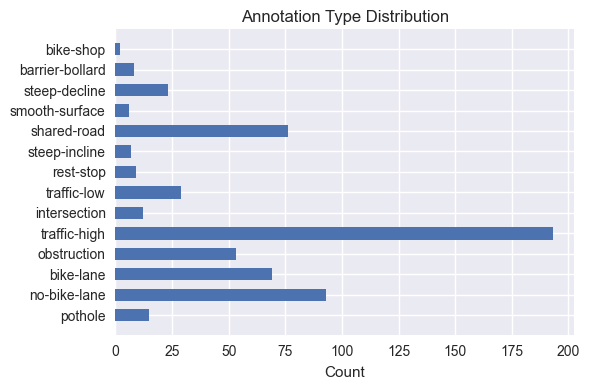
\includegraphics[width=1\linewidth]{figures/chapt6/Dataset_AnnotationDistribution.png}
    \caption{Distribution of annotation types in the WeCyclePH dataset, showing the proportion of user- and system-generated annotations among the 4,169 recorded ride segments, with 595 total annotations across various categories.}
    \label{fig:Dataset_annotation-distribution}
\end{figure}

Across all segments, the dataset spans a cumulative distance of \textbf{682 kilometers}, with a combined ride duration of over \textbf{43 hours}. The average speed across all segments is approximately \textbf{3.39 meters per second}, with a total elevation gain of \textbf{7,432 meters}.

This summary demonstrates that the dataset not only captures a wide range of geographic and environmental conditions but also supports analysis of traffic patterns, road safety infrastructure, and terrain variability. The inclusion of both annotated and non-annotated segments enables balanced quantitative and qualitative evaluations.

\section{Applications}

The WeCyclePH dataset supports a broad spectrum of use cases:

\begin{itemize}
    \item Infrastructure audits identifying gaps in bike lane coverage.
    \item Community reports showing cyclist sentiment per road segment.
    \item Visual dashboards for hazard mapping and hot spot detection.
    \item Routing tools that recommend smoother, safer paths.
    \item Training data for machine learning models on urban navigation.
\end{itemize}

Our segment-centric structure encourages modular analysis. A policymaker might examine segments tagged frequently with \texttt{no-bike-lane} to plan interventions. An activist group might visualize \texttt{obstruction} reports to lobby for cleaner routes.

This dataset is not a static artifact; it is a living map of how people move through cities and what they encounter. Its combination of spatial geometry and qualitative insight is what sets it apart.

\section{Limitations}

 The dataset generated through the WeCyclePH platform provides a rich representation of cycling experiences across multiple geographic regions, however, several limitations must be acknowledged regarding its scope, completeness, and structure.

\subsection{Geographic Coverage and Sampling Bias}

The dataset is inherently shaped by the geographic distribution of participating cyclists. Although contributions were received from regions including Metro Manila, Calabarzon, Zamboanga Peninsula, and the Cordillera Administrative Region, the density of ride data is uneven. Areas with more active cycling communities or stronger recruitment efforts are more heavily represented, while regions with lower cyclist engagement remain underrepresented. This uneven coverage can introduce spatial bias in any downstream analysis, particularly if findings are generalized to a broader national context.

Participation was voluntary and dependent on users' willingness and ability to record their rides. This inherently favors more engaged cyclists, often those with access to smartphones, GPS-enabled devices, and reliable internet connections. Consequently, the dataset may under-represent the experiences of occasional cyclists, low-income riders, or individuals cycling in areas with poor digital infrastructure.


\subsection{Temporal Coverage}

The dataset reflects rides recorded during the defined data collection period, which was limited in duration. As such, it may not capture seasonal variations in cycling conditions, temporal shifts in traffic patterns, or infrastructure changes occurring after the study period. Analysis based on this dataset should therefore be understood as a snapshot in time rather than a continuously updated representation of cycling conditions.

\subsection{Annotation Variability}

Although annotation categories were standardized during preprocessing, the quality and completeness of user-submitted annotations remain subject to variability. Cyclists may differ in their interpretation of annotation categories (e.g., what constitutes “high traffic” versus “shared road”), and some may omit annotations altogether despite encountering relevant conditions. While the inclusion of predefined annotation classes in later iterations reduced this variability, inconsistencies remain, especially in early contributions.

\subsection{Media Contributions}

Not all ride segments are accompanied by media uploads, and where media exists, it is unevenly distributed across the dataset. Video and photo evidence can provide valuable context for annotations, but their absence in many records limits the ability to visually verify all reported conditions. Furthermore, media files are stored externally and linked through URIs, meaning that long-term accessibility depends on maintaining those storage systems.

\subsection{Data Completeness and Sensor Accuracy}

GPS accuracy can vary significantly based on environmental factors such as urban canyon effects, atmospheric conditions, or device hardware limitations. This variability can introduce minor positional errors in the recorded routes, potentially affecting the precision of segment-level metrics such as distance, speed, and elevation gain. Elevation data, in particular, is often less reliable on consumer-grade devices, and calculated elevation gain values should be interpreted with caution.

\subsection{Segment-Level Structuring}

While segmenting rides into directionally consistent portions improves the granularity of analysis, it also means that some contextual continuity is lost between segments. For example, a hazard encountered just after a sharp turn will appear in a separate segment from the preceding portion of the ride, even though the cyclist may perceive it as part of the same continuous experience. Analysts using the dataset should be aware of this segmentation logic when interpreting results.

\subsection{Compatibility with Other Platforms}

While the WeCyclePH dataset shares the common goal of representing geographic information, it is not directly compatible with the formats or schemas used in OpenStreetMap (OSM). OSM's primary exports are provided in XML-based \texttt{.osm} files, organized around three core elements: nodes, ways, and relations. These elements store coordinates and topological relationships, accompanied by a flexible tagging system (e.g., highway=cycleway, surface=asphalt) to describe infrastructure attributes.

In contrast, the WeCyclePH dataset is stored as a GeoJSON FeatureCollection, where each feature is a \texttt{LineString} representing a continuous cycling route segment. Rather than static infrastructure, each segment is derived from actual ride traces collected via GPS and is enriched with dynamic, cyclist-contributed information: segment-level performance metrics (distance, duration, average speed, elevation gain), qualitative annotations (hazard type, perceived safety, sentiment), and optional media references.

Although there are open-source tools such as osmtogeojson that can convert OSM data into GeoJSON, these outputs preserve OSM's tag-based schema and do not directly align with the structure of WeCyclePH's dataset. Likewise, mapping WeCyclePH's features into OSM would require a schema harmonization process, since OSM does not have native tag equivalents for many of the experience-based attributes in WeCyclePH.

This difference limits the dataset's interoperability for direct use in OSM editing or automated updates. However, the dataset is fully compatible with modern web mapping platforms such as Leaflet and Mapbox, which natively accept GeoJSON as an input format. Without any transformation, the dataset can be loaded into these platforms for visualization, spatial filtering, and interactive analysis. This makes the WeCyclePH dataset immediately usable for applications such as hazard heatmaps, route condition overlays, and infrastructure planning dashboards - providing actionable insights even without OSM integration.

Thus, while direct integration into OSM's ecosystem is limited without schema transformation, the dataset retains broad applicability across geospatial visualization and analysis platforms, allowing it to complement existing base maps and enhance cycling-related decision-making.